% !Mode:: "TeX:UTF-8"
%%% Local Variables:
%%% mode: latex
%%% TeX-master: t
%%% End:

% 绪论和国内外现状

\chapter{绪论}
\label{cha:intro}
近些年来,随着互联网的快速发展,人工智能和大数据技术的兴起和应用,网络数据、信息和知识大量增长。
传统的基于网页链接检索的信息存储、信息检索方式越来越难于进行查找学习知识,随着移动设备
的增加,人们对于信息检索、知识获取的要求也越来越高,面对各种数据信息,
人们查找检索知识的需求越来越迫切,越来越期望能更好更快的检索了解学习知识。
随之知识库构建、推理和应用变得流行起来,越来越多的大学、科研机构和商业公司开始构建大规模知识库,如Google Knowledge Graph\cite{Dong},NELL\cite{NELL-aaai15},YAGO\cite{Suchanek:2007:YCS:1242572.1242667},
Freebase\cite{Bollacker2008FreebaseAC},DBpedia\cite{Bizer:2009:DCP:1640541.1640848}等。
这些知识库基于自动和半自动的信息抽取、众包、专家领域内知识等进行构建,
把互联网、书籍、数据库等各处非结构化的文本中数据结构化、抽取构建知识库,
获得了大量的实体、关系和属性信息,能为人们提供的方便快捷的信息查询、检索、知识学习途径。
这类知识库的数据完整性、数据精确性和数据质量等衡量指标非常高,
已经有很多基于知识库的系统被成功用于商业领域,如谷歌搜索引擎\footnote{https://googleblog.blogspot.com/2012/05/introducing-knowledge-graph-things-not.html},
微软的必应搜索\footnote{https://blogs.bing.com/search/2013/03/21/understand-your-world-with-bing/}等。
除了这些通用领域的知识库之外,也有很多领域知识库被构建和应用,知识库也被用于生物学\cite{Dumontier:2014:BRL:2878453.2878554}、金融学、教育学等各个领域,一些较为成熟的问答系统、个人手机助手如Siri、Google Assistant、微软小冰等也将知识库集成其中。

图\ref{kb}是一个简单的知识库例子,常见的知识库可以用有向图进行逻辑上的可视化表示。
图中展示了实体、实体和实体之间关系,其中实体是描述现实中实际存在的事物、地点、人物、事件如:北京师范大学、北京等,关系是描述实体和实体之间存在的某种联系和特征,如北京师范大学和北京存在着位于的关系。除此之外,
一个知识库中的三元组还可以分为关系型三元组和实体属性三元组。关系三元组典型的例子如:北京师范大学,位于,北京。其中“北京师范大学”和“北京”是实体,
属性事实三元组如:北京,人口,2150万。
其中“北京”是实体,“2150万”是描述实体属性的属性值,“人口”是北京这类实体具有的一种属性类型。
通常关系型三元组用来描述实体和实体之间的联系,实体属性三元组描述实体的属性事实特征,这些不同类型的三元组共同构成一个完整的知识库。

\begin{figure}[H]
\begin{center}
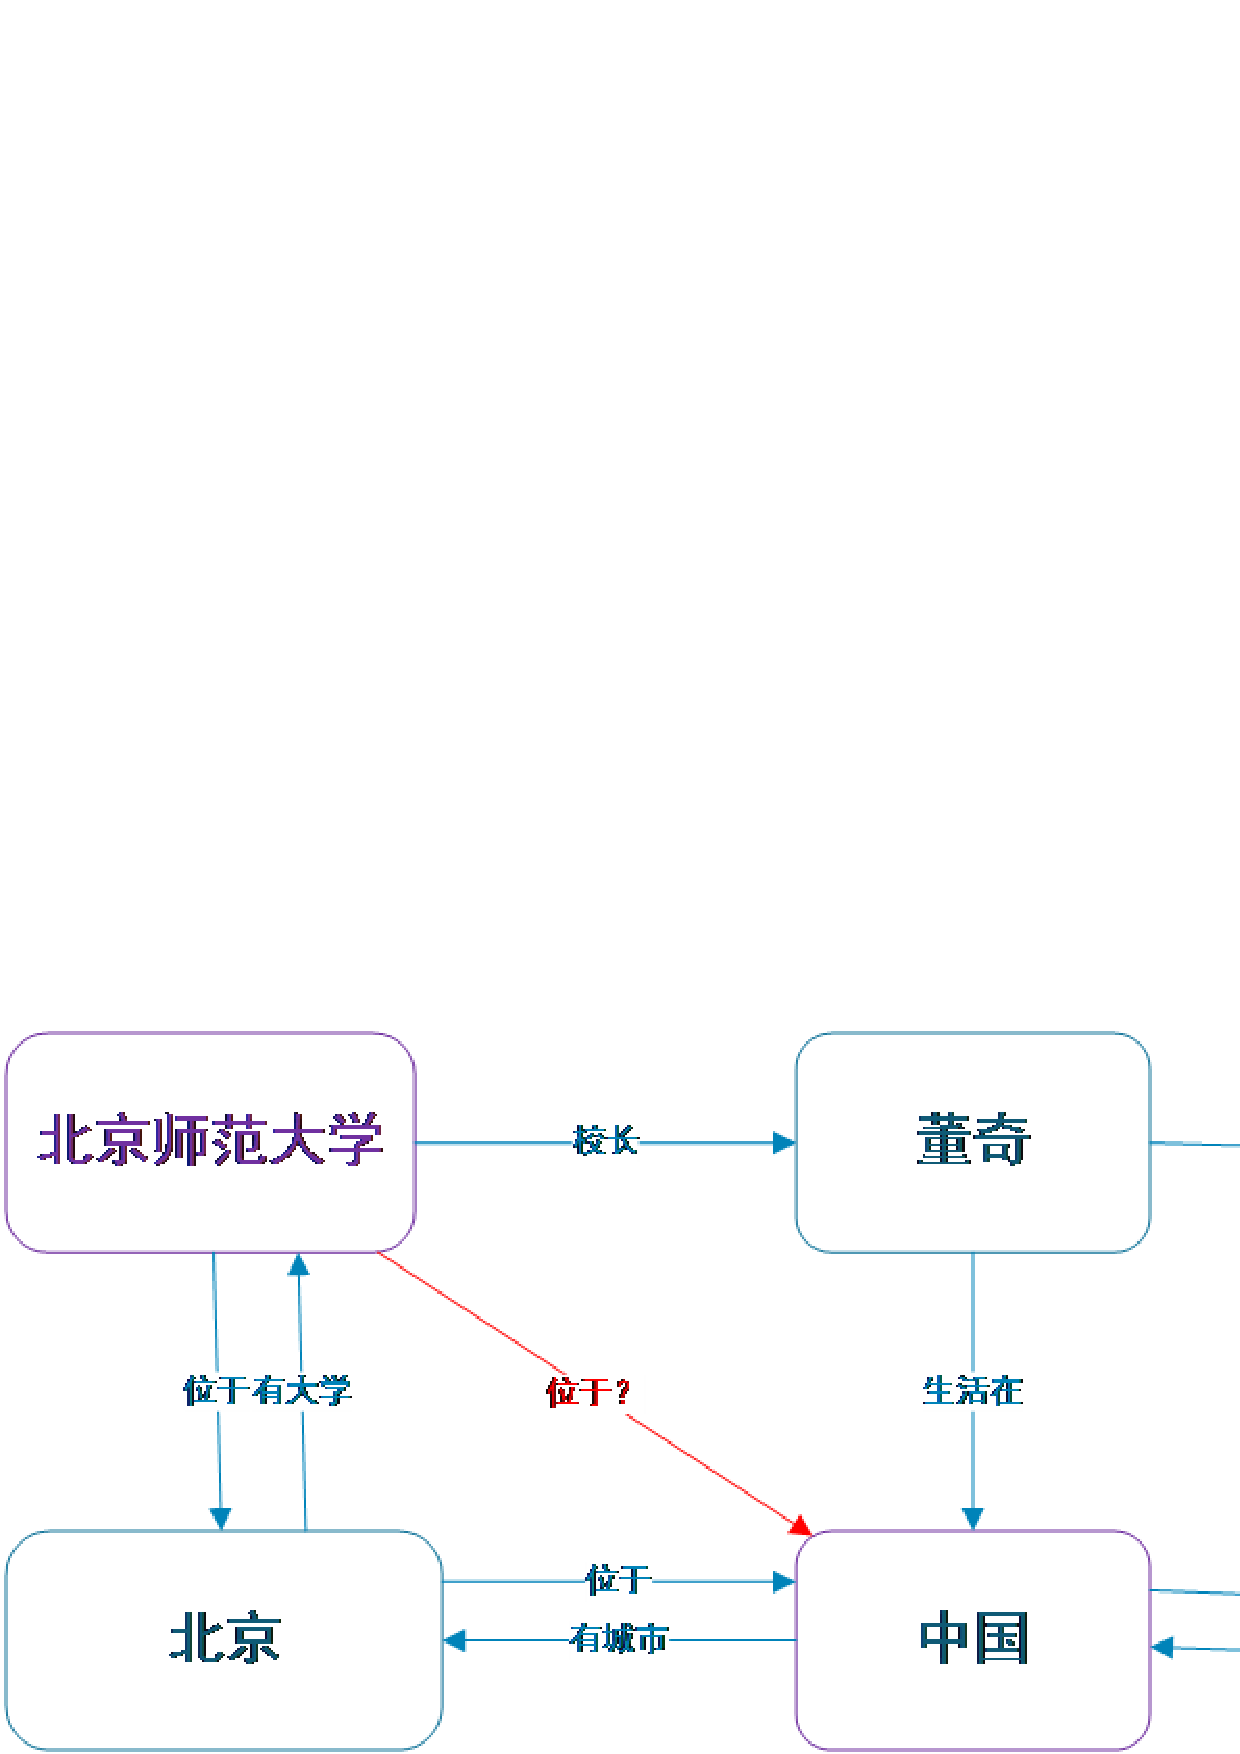
\includegraphics [width=0.5\textwidth]{kb.png}
\caption{一个知识库例子}
\label{kb}
\end{center}
\end{figure}

当前知识库相关的研究主要分为三个方面:(1)知识库的构建,各种基于互联网的、通用的、领域内的知识库构建。
(2)关系机器学习,基于已经构建好的知识库进行关系预测,知识库补全推理等。(3)知识库应用系统。如基于知识库的问答系统,
基于知识库的信息检索系统,生物、金融、教育等领域的本体知识库等。其中研究的热点之一就是知识库补全推理,即如何发掘知识库图结构中隐藏的关系。

当前存在的知识库系统如NELL、Knowledge Vault等,尽管已经包含了大量的实体、关系和属性,但这类知识库中很多实体和实体之间的关系任然是缺失的。例如,尽管知识库中存在很多三元组如:北师大,位于,北京;北京,位于,中国。但是当预测北师大是否位于中国时,通常计算机很难直接进行这类常识性的推理。如何构建一个辅助计算机进行常识推理系统,发现知识库中隐藏的实体和实体之间的关系,是知识库补全系统的重要任务之一。很多基于表示学习和基于符号逻辑的知识库补全算法被提出,这类算法都是基于知识库中现有的关系类型去预测知识库中未知的关系。但是在知识库中存在大量的属性事实型三元组未被使用,而这些属性事实三元组在进行关系预测时有很重要的作用,如:A,isMarriedTo,B,A,HasChild,C。当预测B是否是C的父母时,这些相关实体的年龄、性别等实体属性也很重要。

在构建知识库补全系统的过程中,基于符号逻辑的算法通常通过训练一个二分类的分类器来判断实体和实体之间是否具有某种关系。通常这个分类器的正例是通过抽取现有知识库中存在的三元组作为正例,或称之为正例三元组,而负例则是采用随机采样等方法生成负例三元组。通常在知识库补全系统中,每个正例三元组可以获得上万种不同的负例三元组,如何解决正负例三元组不均衡的问题,正确预测实体和实体之间的关系,也是知识库补全算法的一个重要优化方向。

\section{知识库构建}
在知识库构建过程中,数据完整性、数据精确性和数据质量是构建知识库的重要指标,
通常知识库可以由三元组组成。知识库的构建可以有多种方法:
(1)通过机器学习和自然语言处理技术自动抽取三元组\cite{Weikum2010FromIT}进行构建。
(2)半自动抽取的方法,通过从维基百科等网站的infobox基于规则模式抽取三元组。
(3)基于协同创作\cite{Vrandecic2014WikidataAF}的方法,通过众包的形式系统创建知识库。
(4)基于专家知识构建的领域内知识图谱,这些领域知识图谱有较高的专业性。

\subsection{YAGO知识库}
YAGO是一个从维基百科上抽取的、包含地理名词、WordNet\cite{Kasneci2008TheYA}等数据的知识库。
YAGO将WordNet的词汇定义与维基百科的分类体系进行了融合集成\cite{Suchanek2008YAGOAL},使得YAGO具有更加丰富的实体分类体系。YAGO还考虑了时间和空间知识\cite{Hoffart2011YAGO2EA},为很多知识条目增加了时间和空间维度的属性描述。目前,YAGO包含1.2亿条结合关系三元组和实体属性三元组的知识。YAGO也是IBM Watson\cite{Ferrucci2010BuildingWA}的后端知识库之一。
YAGO2\cite{Hoffart2013YAGO2AS}是YAGO的一个实例,当前YAGO2包括超过260万的实体和超过1.2亿的关系三元组知识,我们使用了其中实体的关系型三元组和属性型三元组共有4,484,914条、
37种关系型三元组的事实描述,同时有3,353,659条、35种属性性三元组的事实描述。

\subsection{Freebase知识库}
Freebase\cite{Bollacker2008FreebaseAC}是一个协同创作的知识库系统,内容通过用户添加,所有的条目采用结构化的形式,将结构分为三次:领域-类型-主题,其中,每一个条目叫做一个主题,每个主题包含不同的属性类型,一些同类型的主题组成一个类型,所有相关的类型构成一个领域。
这种通过协同创作方式创建了结构化的人类知识,截止2007年Freebase包含1.25亿条三元组,超过4000种类型和超过7000种属性知识。一些基于Freebase研究结构化知识的问答系统\cite{Yao2014InformationEO}\cite{Yao2015LeanQA},关注Freebase中的信息抽取和语义解析\cite{Yao2014FreebaseQI},一些研究关注Freebase中的实体消除歧义问题\cite{Zheng2012EntityDW}。

\section{知识库应用}
知识库最广泛的应用是谷歌和微软等商业公司的信息检索系统。2014年谷歌提出的知识图谱\cite{Dong2014KnowledgeVA}就是
结合FreeBase和互联网数据进行信息抽取,知识整合后的著名系统,谷歌也在其博客上讲述了如何将知识库应用在实际的检索中,
微软的Satori也是一个类似的知识库系统,被必应搜索广泛应用。其他搜索公司如百度、搜狗等公司都在知识库构建和信息检索领域有各自的应用。

基于知识库的问答系统也有广泛的发展。2000年就有人提出基于知识的问答系统\cite{HERMJAKOB2000KnowledgeBasedQA}。
有很多方法基于知识库进行表示学习\cite{Yang2014JointRE},然后构建相关的知识库问答系统。还有一些基于标签语义解析的方法,
构建知识库问答系统\cite{Yih2016TheVO}。
一些论文\cite{Yu2017ImprovedNR}研究结合深度学习、关系抽取和问答系统,从而获得更好的知识库问答效果。
一些论文\cite{KeySun2016OpenKB}研究基于开放的知识库构建开放领域的问答系统,期望能基于百科知识进行问答系统构建。
也有基于知识库的系统通过结合智能计算\cite{Pandey2009KnowledgeAI},在医疗诊断领域获得一些突破。
也有一些研究结合了知识库和医疗图像信息\cite{Halpern2014EvaluationOC},对一些医疗疾病进行诊断治疗,期望能获得更好的治疗效果。

\section{知识库补全和推理}
虽然许多知识库的规模很大,但他们仍然是不完备的,如很多人的出生地点并未包含在知识库中,
一些演员是否出演过某些电影也是未知的。为了解决这个问题,很多知识库补全的方法被提出来,
这类方法基于知识库中已有的三元组预测新的三元组,如果将现有的知识库数据看做是多种关系构成的图,
图的顶点是实体,图的边是实体对之间的关系,知识图谱补全可以看成是图中关系的预测。
很多经典的知识库补全算法被提出,这些算法可以分为两类:基于逻辑符号推理的补全算法和基于表示学习的补全算法,
有时候也被称为基于图特征和基于隐藏特征的补全算法。

我们研究了常见的YAGO知识库,发现总共有四百多万实体关系数据被和三百多万属性事实的三元组。
其中的实体关系数据在以往经典的知识库补全算法中被广泛使用,而属性事实数据尽管大量存在,
却在知识库补全系统中并没有得到广泛应用,
同时实体属性数据类型单位差别很大,难以进行统一有效的处理,将这些实体属性特征作为知识库补全的特征也十分困难。
但可以预见在知识库关系预测中,实体属性特征会起着重要的作用,
如何将实体属性三元组有效用于知识库补全是本论文的关键点之一。

此外知识库中的图是稀疏的,每个存在的正例三元组实体对在训练模型中,
可能生成上百组负例三元组实体对,如何解决正负实体对不匹配的问题很关键,在正负实体对比例悬殊时,
关系预测中仅靠逻辑符号推理中的打分模型是不够的,在结果评价中并未考虑候选实体对的顺序对预测结果的影响,
也不关注候选实体的秩序关系,这也是知识库补全算法中需要解决的难点之一。

针对现有知识库补全技术不足,本发明将知识库中的关系路径特征和实体属性特征相结合,构建了一个更准确的知识库补全模型。首先,基于 经典的路径排序模型抽取了关系路径特征;其次通过结合实体属性特征和关系路径特征,构建逻辑回归模型进行关系预测,从而进行知识库补全。
除此之外,本研究提供一种基于学习排序算法的知识库补全技术,
我们通过计算候选头实体和尾实体在关系预测中的位置排序,通过优化排序损失函数MAP来保证训练误差最小,
从而获得最优的关系预测结果,并选择合适的模型评价指标来评估改进我们的预测结果。

